\section{Audit Discrepancies and taxpayer dissatisfaction with the audit process.}
\label{sec:audit_discrepancy_taxpayer}
\providecommand{\sym}[1]{\ifmmode^{#1}\else\(^{#1}\)\fi}

\makeatletter
\@ifundefined{landscape}{\newenvironment{landscape}{}{}}{}
\makeatother

This section studies whether larger discrepancies between notified and confirmed audit amounts are associated with taxpayer-reported efficiency and corruption perceptions.

\subsection{Current empirical steps (updated main specification)}
\begin{enumerate}
\item Start from \texttt{datasetforanalysis.dta}.
\item Keep the broad analysis sample (no ex-ante drop of safety/ad hoc groups), and account for method composition in the regression controls.
\item Recreate cluster groups used in fixed effects:
\begin{verbatim}
capture drop clusterid
egen clusterid = group(inspectorclusteryear)
\end{verbatim}
\item Recreate Table C5 dispute variables (\texttt{d1}--\texttt{d21}) exactly as in the main analysis script.
\item Construct the baseline discrepancy regressor:
\[
W_{\text{main}}=\frac{\text{notificationvalue}-\text{confirmationvalue}}{\text{notificationvalue}}
\]
\item Cap negative baseline values to zero:
\begin{verbatim}
replace W_main = 0 if W_main < 0 & W_main != .
\end{verbatim}
\item Build robustness discrepancy regressors:
\begin{verbatim}
W_nonzero = 1{W_main != 0}
W_abovemed = 1{W_main > median(W_main)}
W_topquart = 1{W_main >= p75(W_main)}
\end{verbatim}
where \(\text{median}(W_{\text{main}})\) and \(p75(W_{\text{main}})\) are single pooled moments from non-missing \(W_{\text{main}}\) in the regression-eligible sample.
\item In exported regression tables, coefficient labels are:
\textit{Downward revision (\% of notification)},
\textit{Downward revision (\% of notification) $\neq 0$},
\textit{Downward revision (\% of notification) $>$ median}, and
\textit{Downward revision (\% of notification) in top quartile}.
\item Build panel indicators:
\begin{verbatim}
selfreported_audit = 1 if q28a in [2018,2021] or q29a in [2018,2021]
\end{verbatim}
Panel A uses \texttt{q1 $\neq$ . AND selfreported  = 1}; Panel B uses \texttt{q1 $\neq$ .}.
\item Build index outcomes as in taxpayer-survey code:
\begin{verbatim}
index_efficiency  from q31 q33 q41
index_corruption  from q32_inverted q42 q34   (swindex)
\end{verbatim}
\item Estimate Table 6 / D7-style columns by audit type (full, desk, all), using method controls:
\begin{verbatim}
W_main algorithm overlap random safeties horsprogramme
\end{verbatim}
Index outcomes use \texttt{a(selectionyear center)}; question outcomes (\texttt{q34 q35 q32 q42}) use \texttt{a(inspectorclusteryear)}. The same backbone is used for the three robustness \(W\) variants.
\end{enumerate}

\subsection{Regression equation and notation}

Our empirical exercise studies whether larger discrepancies between the notified and confirmed audit amounts are associated with taxpayer-reported perceptions of the audit process. Concretely, for each taxpayer-survey outcome, we estimate the following model via Ordinary Least Squares:
\[
y_{ig}
=
\beta_0
+ \beta_1 W_i
+ \beta_2 \text{Algorithm}_i
+ \beta_3 \text{Overlap}_i
+ \beta_4 \text{Random}_i
+ \beta_5 \text{Safeties}_i
+ \beta_6 \text{Horsprogramme}_i
+ \gamma_g
+ \varepsilon_{ig},
\]
where \(y_{ig}\) is the taxpayer-survey outcome for firm-audit observation \(i\), and \(\gamma_g\) denotes the relevant fixed effects. The unit of observation is a firm-audit observation in the merged administrative audit and taxpayer-survey data, so a given firm may appear more than once if it is associated with multiple audit cases.

Our main discrepancy regressor is
\[
W_i
=
\max\left\{
\frac{\text{Notification}_i-\text{Confirmation}_i}{\text{Notification}_i},
\,0
\right\},
\]
defined for observations with strictly positive notified and confirmed amounts and an executed audit. Thus, \(W_i=0\) both when there is no positive discrepancy and when the confirmed amount is at least as large as the notified amount.

The indicators \(\text{Algorithm}_i\), \(\text{Overlap}_i\), \(\text{Random}_i\), \(\text{Safeties}_i\), and \(\text{Horsprogramme}_i\) capture the audit-case classification. The dummy for random selection is applicable only to desk-audit specifications. The coefficient of interest is \(\beta_1\), which captures the association between the capped discrepancy measure and the taxpayer-reported outcome.

We estimate this equation separately by panel and audit type. Panel A restricts the sample to firms that report having been audited recently,
\[
\texttt{q1 != . \& selfreported\_audit == 1},
\]
while Panel B includes all surveyed firms with non-missing \texttt{q1},
\[
\texttt{q1 != .}.
\]
For audit type, we estimate the specification separately for full audits (\texttt{x2 == 1}), desk audits (\texttt{x2 == 0}), and the pooled sample with no restriction on \texttt{x2}.

The outcomes are the taxpayer-survey indices
\[
\texttt{index\_efficiency}, \quad \texttt{index\_corruption},
\]
and the individual survey questions
\[
\texttt{q34}, \quad \texttt{q35}, \quad \texttt{q32}, \quad \texttt{q42}.
\]
For index outcomes, the fixed effects \(\gamma_g\) correspond to \texttt{selectionyear} \(\times\) \texttt{center}. For question-level outcomes, \(\gamma_g\) corresponds to \texttt{inspectorclusteryear}. We use robust standard errors to perform inference.

In robustness checks, we also replace \(W_i\) with indicator versions:
\[
W_i^{\neq 0}=\mathbf{1}\{W_i\neq 0\},
\qquad
W_i^{>\mathrm{med}}=\mathbf{1}\{W_i>\widetilde{W}\},
\qquad
W_i^{\ge q75}=\mathbf{1}\{W_i\ge\widetilde{W}_{75}\},
\]
where \(\widetilde{W}\) is the pooled median and \(\widetilde{W}_{75}\) is the pooled 75th percentile of non-missing \(W_i\) in the relevant regression sample.

\subsection{Coverage and \(W\) diagnostics}

\begin{table}[!htbp]
\centering
\resizebox{\textwidth}{!}{%
\begin{threeparttable}
\caption{Informative regression-sample coverage by panel and audit type (counts and \% of base)}
\begin{tabular}{l*{6}{c}}

                    &\multicolumn{3}{c}{Panel A: Recent audit}&\multicolumn{3}{c}{Panel B: All surveyed}\\
                    &\multicolumn{1}{c}{Full audits}&\multicolumn{1}{c}{Desk audits}&\multicolumn{1}{c}{All audits}&\multicolumn{1}{c}{Full audits}&\multicolumn{1}{c}{Desk audits}&\multicolumn{1}{c}{All audits}\\
\hline
Eligible surveyed firms (q1 observed)&         227&         413&         640&         262&         501&         763\\
Executed cases (y2=1)&         107&         181&         288&         120&         229&         349\\
Non-missing W       &          54&          62&         116&          59&          76&         135\\
Non-missing W + method controls&          54&          62&         116&          59&          76&         135\\
Regression sample: Efficiency index&          54&          59&         113&          58&          70&         128\\
Regression sample: Corruption index&          53&          59&         112&          57&          71&         128\\
Regression sample: Corruption in General (q34)&          40&          36&          76&          43&          44&          87\\
Regression sample: Corruption Experience (q35)&          54&          62&         116&          59&          75&         134\\
Regression sample: Grade on Honesty (q32)&          49&          52&         101&          52&          59&         111\\
Regression sample: Friend at tax Auth. (q42)&          50&          51&         101&          52&          61&         113\\
\hline

\end{tabular}
\begin{tablenotes}[flushleft]
\footnotesize
\item Notes: Coverage rows report counts and percentages relative to the base surveyed sample in each panel-column cell (base \(=\) firms with \(q1\) observed). Panels are defined as in the regression tables.
\end{tablenotes}
\end{threeparttable}
}
\end{table}

\begin{figure}[!htbp]
\centering
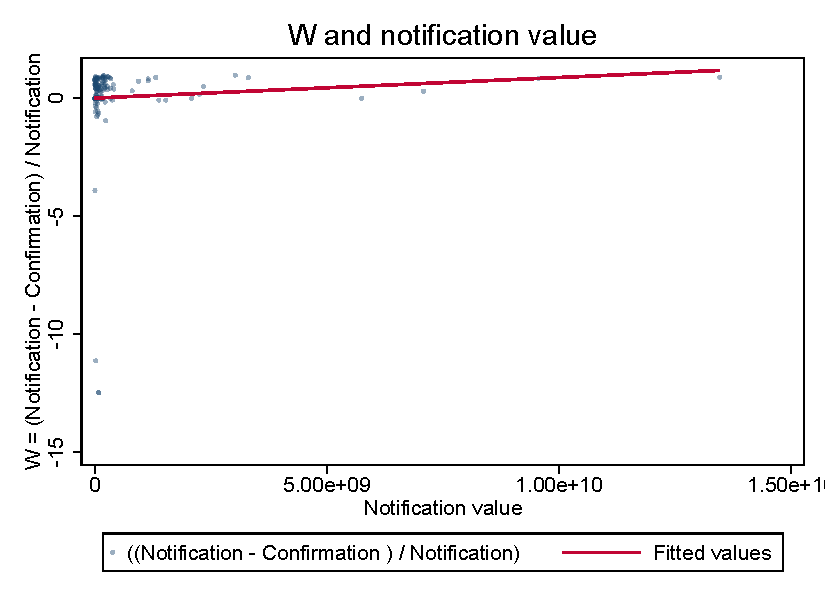
\includegraphics[width=0.82\textwidth]{Output/w_main_scatter_notification.pdf}
\caption{Scatter and linear fit: \(W_{\text{main}}\) vs notification value}
\end{figure}

\begin{figure}[!htbp]
\centering
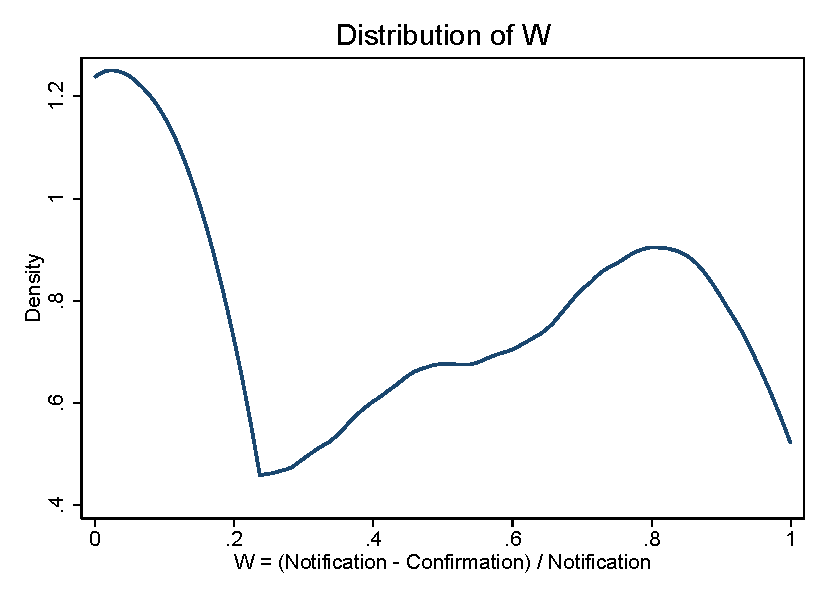
\includegraphics[width=0.75\textwidth]{Output/w_main_density.pdf}
\caption{Density of \(W_{\text{main}}\)}
\end{figure}

\subsection{Main regression tables (current outputs)}

\begin{table}[!htbp]
\centering
\resizebox{\textwidth}{!}{%
\begin{threeparttable}
\caption{Selection method, capped \(W\), and survey indexes: two panels (Recent audit / All surveyed firms)}
\begin{tabular}{l*{6}{c}}
\textbf{A: Surveyed Firms (Self-Reporting a Recent Audit)}
                    &\multicolumn{3}{c}{Efficiency Index}                             &\multicolumn{3}{c}{Corruption Index}                             \\
                    &\multicolumn{1}{c}{(1)}&\multicolumn{1}{c}{(2)}&\multicolumn{1}{c}{(3)}&\multicolumn{1}{c}{(4)}&\multicolumn{1}{c}{(5)}&\multicolumn{1}{c}{(6)}\\
                    &\multicolumn{1}{c}{Full audits}&\multicolumn{1}{c}{Desk audits}&\multicolumn{1}{c}{All audits}&\multicolumn{1}{c}{Full audits}&\multicolumn{1}{c}{Desk audits}&\multicolumn{1}{c}{All audits}\\
\hline
W                   &        0.20         &       -0.01         &        0.06         &        0.30         &       -0.00         &       -0.02         \\
                    &      (0.43)         &      (0.05)         &      (0.05)         &      (0.37)         &      (0.04)         &      (0.03)         \\
[1em]
Algorithm           &       -0.53         &        0.44         &       -0.13         &        0.30         &       -0.38         &       -0.03         \\
                    &      (0.35)         &      (0.33)         &      (0.24)         &      (0.28)         &      (0.29)         &      (0.22)         \\
[1em]
Inspectors x Overlap&        0.17         &       -0.76         &       -0.52         &        0.65\sym{*}  &       -0.41         &        0.30         \\
                    &      (0.39)         &      (0.53)         &      (0.46)         &      (0.37)         &      (0.46)         &      (0.30)         \\
[1em]
Algorithm x Random  &                     &       -0.17         &       -0.01         &                     &       -0.15         &       -0.13         \\
                    &                     &      (0.30)         &      (0.30)         &                     &      (0.35)         &      (0.26)         \\
\hline
N                   &          51         &          59         &         113         &          50         &          59         &         112         \\
R2                  &        0.11         &        0.32         &        0.12         &        0.27         &        0.39         &        0.17         \\
Mean outcome        &        0.00         &       -0.06         &       -0.02         &       -0.15         &       -0.10         &       -0.11         \\
\hline
\textbf{B: All Surveyed Firms}
                    &\multicolumn{1}{c}{(1)}         &\multicolumn{1}{c}{(2)}         &\multicolumn{1}{c}{(3)}         &\multicolumn{1}{c}{(4)}         &\multicolumn{1}{c}{(5)}         &\multicolumn{1}{c}{(6)}         \\
\hline
W                   &        0.27         &        0.01         &        0.07         &        0.11         &       -0.01         &       -0.03         \\
                    &      (0.40)         &      (0.05)         &      (0.04)         &      (0.34)         &      (0.04)         &      (0.03)         \\
[1em]
Algorithm           &       -0.54         &        0.19         &       -0.22         &        0.38         &       -0.38         &       -0.01         \\
                    &      (0.34)         &      (0.29)         &      (0.22)         &      (0.27)         &      (0.28)         &      (0.21)         \\
[1em]
Inspectors x Overlap&        0.25         &       -0.92\sym{**} &       -0.48         &        0.52         &       -0.16         &        0.27         \\
                    &      (0.37)         &      (0.40)         &      (0.47)         &      (0.36)         &      (0.43)         &      (0.28)         \\
[1em]
Algorithm x Random  &                     &       -0.16         &       -0.05         &                     &       -0.19         &       -0.11         \\
                    &                     &      (0.28)         &      (0.26)         &                     &      (0.34)         &      (0.25)         \\
\hline
N                   &          55         &          70         &         128         &          54         &          71         &         128         \\
R2                  &        0.14         &        0.28         &        0.14         &        0.26         &        0.25         &        0.12         \\
Mean outcome        &        0.00         &        0.01         &        0.02         &       -0.18         &       -0.06         &       -0.10         \\
\hline

\end{tabular}
\begin{tablenotes}[flushleft]
\footnotesize
\item Notes: OLS results for the Efficiency Index and Corruption Index. The specification is \(y_{ig}=\beta_0+\beta_1 W_i+\beta_2 \text{Algorithm}_i+\beta_3 \text{Overlap}_i+\beta_4 \text{Random}_i+\beta_5 \text{Safeties}_i+\beta_6 \text{Horsprogramme}_i+\gamma_g+\varepsilon_{ig}\). Here \(W_i=W_{\text{main},i}=\max\{(notificationvalue_i-confirmationvalue_i)/notificationvalue_i,0\}\). The control set follows Table D7 (algorithm-selection, overlap, random-selection, replacement, and ad hoc indicators), with the addition of \(W_i\). Panel A includes surveyed firms that report having been audited recently; Panel B includes all surveyed firms. Within each panel, columns report full audits, desk audits, and all audits. Fixed effects are at the selection-year \(\times\) tax-office level. Robust standard errors (Huber-White) are in parentheses. Stars denote significance at \(^{*}p<0.10\), \(^{**}p<0.05\), \(^{***}p<0.01\).
\end{tablenotes}
\end{threeparttable}
}
\end{table}

\begin{landscape}
\begin{table}[!htbp]
\centering
\resizebox{\textwidth}{!}{%
\begin{threeparttable}
\caption{Selection method, capped \(W\), and survey-question outcomes: two panels (Recent audit / All surveyed firms)}
\begin{tabular}{l*{12}{c}}
\textbf{A: Surveyed Firms (Self-Reporting a Recent Audit)}
                    &\multicolumn{3}{c}{Corruption in General}                        &\multicolumn{3}{c}{Corruption Experience}                        &\multicolumn{3}{c}{Grade on Honesty}                             &\multicolumn{3}{c}{Friend at tax Auth.}                          \\
                    &\multicolumn{1}{c}{(1)}&\multicolumn{1}{c}{(2)}&\multicolumn{1}{c}{(3)}&\multicolumn{1}{c}{(4)}&\multicolumn{1}{c}{(5)}&\multicolumn{1}{c}{(6)}&\multicolumn{1}{c}{(7)}&\multicolumn{1}{c}{(8)}&\multicolumn{1}{c}{(9)}&\multicolumn{1}{c}{(10)}&\multicolumn{1}{c}{(11)}&\multicolumn{1}{c}{(12)}\\
                    &\multicolumn{1}{c}{Full audits}&\multicolumn{1}{c}{Desk audits}&\multicolumn{1}{c}{All audits}&\multicolumn{1}{c}{Full audits}&\multicolumn{1}{c}{Desk audits}&\multicolumn{1}{c}{All audits}&\multicolumn{1}{c}{Full audits}&\multicolumn{1}{c}{Desk audits}&\multicolumn{1}{c}{All audits}&\multicolumn{1}{c}{Full audits}&\multicolumn{1}{c}{Desk audits}&\multicolumn{1}{c}{All audits}\\
\hline
W                   &      18.646         &      -0.120         &      -1.620         &      -0.131         &                     &      -0.007         &      -1.085         &       0.141         &       0.047         &      -0.080         &       0.162         &       0.142         \\
                    &    (11.367)         &     (3.229)         &     (1.690)         &     (0.172)         &                     &     (0.011)         &     (0.984)         &     (0.191)         &     (0.196)         &     (0.739)         &     (0.120)         &     (0.101)         \\
[1em]
Algorithm           &      -4.046         &     -44.528         &     -10.484         &       0.031         &                     &       0.025         &      -0.885         &      -2.254         &      -1.152         &       0.198         &      -0.139         &       0.147         \\
                    &     (6.547)         &    (38.381)         &     (7.186)         &     (0.090)         &                     &     (0.080)         &     (0.886)         &     (1.440)         &     (0.817)         &     (0.509)         &     (1.156)         &     (0.484)         \\
[1em]
Inspectors x Overlap&      33.691\sym{***}&                     &      36.936\sym{***}&       0.052         &                     &       0.007         &      -0.648         &                     &      -1.052         &       0.097         &                     &      -0.007         \\
                    &     (4.713)         &                     &     (4.160)         &     (0.064)         &                     &     (0.018)         &     (1.616)         &                     &     (1.719)         &     (0.600)         &                     &     (0.561)         \\
[1em]
Algorithm x Random  &                     &                     &                     &                     &                     &      -0.022         &                     &                     &                     &                     &      -0.918         &      -1.198         \\
                    &                     &                     &                     &                     &                     &     (0.079)         &                     &                     &                     &                     &     (1.423)         &     (0.806)         \\
\hline
N                   &          38         &          10         &          48         &          50         &          34         &          84         &          46         &          24         &          70         &          45         &          25         &          70         \\
R2                  &       0.294         &       0.638         &       0.310         &       0.203         &           .         &       0.207         &       0.195         &       0.478         &       0.248         &       0.156         &       0.593         &       0.318         \\
Mean outcome        &       11.81         &       20.50         &       13.62         &        0.08         &        0.00         &        0.04         &        6.78         &        6.45         &        6.67         &        3.40         &        3.48         &        3.42         \\
\hline
\textbf{B: All Surveyed Firms}
                    &\multicolumn{1}{c}{(1)}         &\multicolumn{1}{c}{(2)}         &\multicolumn{1}{c}{(3)}         &\multicolumn{1}{c}{(4)}         &\multicolumn{1}{c}{(5)}         &\multicolumn{1}{c}{(6)}         &\multicolumn{1}{c}{(7)}         &\multicolumn{1}{c}{(8)}         &\multicolumn{1}{c}{(9)}         &\multicolumn{1}{c}{(10)}         &\multicolumn{1}{c}{(11)}         &\multicolumn{1}{c}{(12)}         \\
\hline
W                   &      10.735         &      -2.130         &      -2.283\sym{*}  &      -0.213         &                     &      -0.011         &      -0.959         &       0.097         &       0.040         &      -0.215         &       0.130         &       0.121         \\
                    &    (11.482)         &     (1.904)         &     (1.314)         &     (0.174)         &                     &     (0.013)         &     (0.957)         &     (0.226)         &     (0.200)         &     (0.696)         &     (0.127)         &     (0.101)         \\
[1em]
Algorithm           &      -5.625         &     -22.938         &     -10.122         &       0.024         &                     &       0.020         &      -0.884         &      -1.065         &      -0.944         &       0.249         &       0.515         &       0.340         \\
                    &     (6.254)         &    (21.168)         &     (6.261)         &     (0.087)         &                     &     (0.068)         &     (0.863)         &     (1.034)         &     (0.731)         &     (0.499)         &     (0.895)         &     (0.444)         \\
[1em]
Inspectors x Overlap&      19.048         &                     &      23.436         &      -0.068         &                     &      -0.158         &      -0.176         &                     &      -0.606         &       0.174         &                     &       0.022         \\
                    &    (16.079)         &                     &    (15.200)         &     (0.149)         &                     &     (0.186)         &     (1.424)         &                     &     (1.412)         &     (0.541)         &                     &     (0.384)         \\
[1em]
Algorithm x Random  &                     &                     &                     &                     &                     &      -0.021         &                     &      -1.763\sym{*}  &      -1.901\sym{**} &                     &      -1.561         &      -1.383\sym{*}  \\
                    &                     &                     &                     &                     &                     &     (0.046)         &                     &     (0.956)         &     (0.918)         &                     &     (1.175)         &     (0.774)         \\
\hline
N                   &          41         &          16         &          57         &          55         &          46         &         101         &          49         &          31         &          80         &          47         &          32         &          79         \\
R2                  &       0.185         &       0.530         &       0.285         &       0.200         &           .         &       0.181         &       0.215         &       0.462         &       0.272         &       0.153         &       0.403         &       0.276         \\
Mean outcome        &       12.78         &       16.87         &       13.92         &        0.09         &        0.00         &        0.04         &        6.77         &        6.51         &        6.67         &        3.36         &        3.75         &        3.51         \\
\hline

\end{tabular}
\begin{tablenotes}[flushleft]
\footnotesize
\item Notes: OLS results for four taxpayer-survey outcomes: Corruption in general (Columns 1 to 3), Corruption experience (Columns 4 to 6), Grade on honesty (Columns 7 to 9), and Friend at tax authority (Columns 10 to 12). The specification is \(y_{ig}=\beta_0+\beta_1 W_i+\beta_2 \text{Algorithm}_i+\beta_3 \text{Overlap}_i+\beta_4 \text{Random}_i+\beta_5 \text{Safeties}_i+\beta_6 \text{Horsprogramme}_i+\gamma_g+\varepsilon_{ig}\). Here \(W_i=W_{\text{main},i}=\max\{(notificationvalue_i-confirmationvalue_i)/notificationvalue_i,0\}\). The control set follows Table D7 (algorithm-selection, overlap, random-selection, replacement, and ad hoc indicators), with the addition of \(W_i\). Panel A includes surveyed firms that report having been audited recently; Panel B includes all surveyed firms. Within each panel, columns report full audits, desk audits, and all audits. Corruption in general is the declared belief about the percentage of audits in Senegal affected by corruption; Corruption experience indicates that the respondent declared an instance of bribery to obtain tax favors; Grade on honesty is a 0-to-10 grade for the honesty of the inspector with whom the respondent last interacted during a full audit; and Friend at tax authority captures agreement with the statement that if the firm's owner has a friend at the tax authority, the firm will rarely be audited. Fixed effects are at the inspector-cluster-year level. Robust standard errors (Huber-White) are in parentheses. Stars denote significance at \(^{*}p<0.10\), \(^{**}p<0.05\), \(^{***}p<0.01\).
\end{tablenotes}
\end{threeparttable}
}
\end{table}
\end{landscape}

\subsection{Robustness regression tables}

\begin{table}[!htbp]
\centering
\resizebox{\textwidth}{!}{%
\begin{threeparttable}
\caption{Robustness: \(W_{\neq 0}\) and survey indexes (Recent audit / All surveyed firms)}
\begin{tabular}{l*{6}{c}}
\textbf{A: Surveyed Firms (Self-Reporting a Recent Audit)}
                    &\multicolumn{3}{c}{Efficiency Index}                             &\multicolumn{3}{c}{Corruption Index}                             \\
                    &\multicolumn{1}{c}{(1)}&\multicolumn{1}{c}{(2)}&\multicolumn{1}{c}{(3)}&\multicolumn{1}{c}{(4)}&\multicolumn{1}{c}{(5)}&\multicolumn{1}{c}{(6)}\\
                    &\multicolumn{1}{c}{Full audits}&\multicolumn{1}{c}{Desk audits}&\multicolumn{1}{c}{All audits}&\multicolumn{1}{c}{Full audits}&\multicolumn{1}{c}{Desk audits}&\multicolumn{1}{c}{All audits}\\
\hline
Downward revision (\% of notification) $\neq$ 0&        0.43         &       -0.07         &        0.21         &        0.29         &        0.21         &        0.15         \\
                    &      (0.41)         &      (0.27)         &      (0.22)         &      (0.33)         &      (0.22)         &      (0.17)         \\
[1em]
Algorithm           &       -0.52         &        0.43         &       -0.12         &        0.31         &       -0.42         &       -0.03         \\
                    &      (0.36)         &      (0.32)         &      (0.24)         &      (0.28)         &      (0.29)         &      (0.21)         \\
[1em]
Inspectors x Overlap&        0.29         &       -1.13\sym{*}  &       -0.68         &        0.68\sym{*}  &       -0.36         &        0.31         \\
                    &      (0.38)         &      (0.63)         &      (0.54)         &      (0.36)         &      (0.35)         &      (0.24)         \\
[1em]
Algorithm x Random  &                     &       -0.01         &        0.04         &                     &       -0.14         &       -0.10         \\
                    &                     &      (0.31)         &      (0.30)         &                     &      (0.32)         &      (0.25)         \\
\hline
N                   &          55         &          81         &         138         &          54         &          81         &         137         \\
R2                  &        0.15         &        0.25         &        0.09         &        0.28         &        0.33         &        0.19         \\
Mean outcome        &       -0.01         &       -0.01         &        0.00         &       -0.13         &       -0.10         &       -0.11         \\
\hline
\textbf{B: All Surveyed Firms}
                    &\multicolumn{1}{c}{(1)}         &\multicolumn{1}{c}{(2)}         &\multicolumn{1}{c}{(3)}         &\multicolumn{1}{c}{(4)}         &\multicolumn{1}{c}{(5)}         &\multicolumn{1}{c}{(6)}         \\
\hline
Downward revision (\% of notification) $\neq$ 0&        0.46         &       -0.08         &        0.18         &        0.08         &        0.21         &        0.09         \\
                    &      (0.35)         &      (0.23)         &      (0.19)         &      (0.31)         &      (0.21)         &      (0.16)         \\
[1em]
Algorithm           &       -0.52         &        0.17         &       -0.20         &        0.37         &       -0.38         &       -0.03         \\
                    &      (0.34)         &      (0.28)         &      (0.22)         &      (0.27)         &      (0.29)         &      (0.21)         \\
[1em]
Inspectors x Overlap&        0.30         &       -1.44\sym{**} &       -0.76         &        0.58         &       -0.17         &        0.41\sym{*}  \\
                    &      (0.33)         &      (0.60)         &      (0.54)         &      (0.35)         &      (0.37)         &      (0.22)         \\
[1em]
Algorithm x Random  &                     &        0.04         &        0.05         &                     &       -0.20         &       -0.16         \\
                    &                     &      (0.29)         &      (0.27)         &                     &      (0.32)         &      (0.25)         \\
\hline
N                   &          61         &          96         &         159         &          60         &          97         &         159         \\
R2                  &        0.18         &        0.20         &        0.09         &        0.30         &        0.22         &        0.12         \\
Mean outcome        &        0.01         &        0.03         &        0.03         &       -0.22         &       -0.05         &       -0.11         \\
\hline

\end{tabular}
\begin{tablenotes}[flushleft]
\footnotesize
\item Notes: OLS results for the Efficiency Index and Corruption Index. The specification is \(y_{ig}=\beta_0+\beta_1 W_i^{\neq 0}+\beta_2 \text{Algorithm}_i+\beta_3 \text{Overlap}_i+\beta_4 \text{Random}_i+\beta_5 \text{Safeties}_i+\beta_6 \text{Horsprogramme}_i+\gamma_g+\varepsilon_{ig}\). Here \(W_i^{\neq 0}=\mathbf{1}\{W_{\text{main},i}\neq 0\}\). The control set follows Table D7 (algorithm-selection, overlap, random-selection, replacement, and ad hoc indicators), with the addition of the discrepancy term \(W_i^{\neq 0}\). Panel A includes surveyed firms that report having been audited recently; Panel B includes all surveyed firms. Within each panel, columns report full audits, desk audits, and all audits. Fixed effects are at the selection-year \(\times\) tax-office level. Robust standard errors (Huber-White) are in parentheses. Stars denote significance at \(^{*}p<0.10\), \(^{**}p<0.05\), \(^{***}p<0.01\).
\end{tablenotes}
\end{threeparttable}
}
\end{table}

\begin{landscape}
\begin{table}[!htbp]
\centering
\resizebox{\textwidth}{!}{%
\begin{threeparttable}
\caption{Robustness: \(W_{\neq 0}\) and survey questions (Recent audit / All surveyed firms)}
\begin{tabular}{l*{12}{c}}
\textbf{A: Surveyed Firms (Self-Reporting a Recent Audit)}
                    &\multicolumn{3}{c}{Corruption in General}                        &\multicolumn{3}{c}{Corruption Experience}                        &\multicolumn{3}{c}{Grade on Honesty}                             &\multicolumn{3}{c}{Friend at tax Auth.}                          \\
                    &\multicolumn{1}{c}{(1)}&\multicolumn{1}{c}{(2)}&\multicolumn{1}{c}{(3)}&\multicolumn{1}{c}{(4)}&\multicolumn{1}{c}{(5)}&\multicolumn{1}{c}{(6)}&\multicolumn{1}{c}{(7)}&\multicolumn{1}{c}{(8)}&\multicolumn{1}{c}{(9)}&\multicolumn{1}{c}{(10)}&\multicolumn{1}{c}{(11)}&\multicolumn{1}{c}{(12)}\\
                    &\multicolumn{1}{c}{Full audits}&\multicolumn{1}{c}{Desk audits}&\multicolumn{1}{c}{All audits}&\multicolumn{1}{c}{Full audits}&\multicolumn{1}{c}{Desk audits}&\multicolumn{1}{c}{All audits}&\multicolumn{1}{c}{Full audits}&\multicolumn{1}{c}{Desk audits}&\multicolumn{1}{c}{All audits}&\multicolumn{1}{c}{Full audits}&\multicolumn{1}{c}{Desk audits}&\multicolumn{1}{c}{All audits}\\
\hline
Downward revision (\% of notification) $\neq$ 0&      17.226\sym{*}  &       3.684         &      10.975         &      -0.014         &       0.099         &       0.038         &       0.419         &       0.044         &       0.281         &       0.655         &       0.656         &       0.629\sym{**} \\
                    &     (9.243)         &    (10.664)         &     (7.172)         &     (0.075)         &     (0.069)         &     (0.050)         &     (0.768)         &     (0.631)         &     (0.532)         &     (0.458)         &     (0.422)         &     (0.315)         \\
[1em]
Algorithm           &      -4.663         &     -28.728         &      -8.520         &       0.025         &      -0.062         &       0.005         &      -0.907         &      -1.165         &      -0.942         &       0.200         &       0.509         &       0.245         \\
                    &     (6.720)         &    (21.678)         &     (7.599)         &     (0.089)         &     (0.071)         &     (0.076)         &     (0.873)         &     (1.234)         &     (0.774)         &     (0.481)         &     (0.782)         &     (0.456)         \\
[1em]
Inspectors x Overlap&      38.446\sym{***}&                     &      37.160\sym{***}&       0.005         &                     &       0.001         &      -0.977         &                     &      -0.986         &       0.067         &                     &       0.082         \\
                    &     (2.649)         &                     &     (3.725)         &     (0.018)         &                     &     (0.015)         &     (1.569)         &                     &     (1.673)         &     (0.499)         &                     &     (0.528)         \\
[1em]
Algorithm x Random  &                     &                     &                     &                     &      -0.287         &      -0.273         &                     &       0.111         &      -1.226         &                     &      -1.650\sym{*}  &      -0.835         \\
                    &                     &                     &                     &                     &     (0.223)         &     (0.195)         &                     &     (1.806)         &     (1.010)         &                     &     (0.950)         &     (0.691)         \\
\hline
N                   &          49         &          45         &          94         &          65         &          89         &         154         &          61         &          67         &         128         &          57         &          76         &         133         \\
R2                  &       0.319         &       0.429         &       0.319         &       0.136         &       0.395         &       0.240         &       0.141         &       0.537         &       0.325         &       0.108         &       0.418         &       0.259         \\
Mean outcome        &       12.63         &       17.33         &       14.88         &        0.07         &        0.04         &        0.05         &        6.68         &        6.44         &        6.56         &        3.45         &        3.35         &        3.39         \\
\hline
\textbf{B: All Surveyed Firms}
                    &\multicolumn{1}{c}{(1)}         &\multicolumn{1}{c}{(2)}         &\multicolumn{1}{c}{(3)}         &\multicolumn{1}{c}{(4)}         &\multicolumn{1}{c}{(5)}         &\multicolumn{1}{c}{(6)}         &\multicolumn{1}{c}{(7)}         &\multicolumn{1}{c}{(8)}         &\multicolumn{1}{c}{(9)}         &\multicolumn{1}{c}{(10)}         &\multicolumn{1}{c}{(11)}         &\multicolumn{1}{c}{(12)}         \\
\hline
Downward revision (\% of notification) $\neq$ 0&       9.151         &      -1.612         &       4.676         &      -0.116         &       0.016         &      -0.049         &       0.228         &       0.047         &       0.192         &       0.527         &       0.498         &       0.505\sym{*}  \\
                    &     (9.581)         &    (10.466)         &     (7.148)         &     (0.094)         &     (0.072)         &     (0.059)         &     (0.692)         &     (0.578)         &     (0.482)         &     (0.424)         &     (0.362)         &     (0.280)         \\
[1em]
Algorithm           &      -6.042         &     -20.476         &      -8.787         &       0.015         &       0.016         &       0.024         &      -0.874         &      -0.380         &      -0.747         &       0.250         &       0.402         &       0.301         \\
                    &     (6.344)         &    (14.568)         &     (6.301)         &     (0.088)         &     (0.069)         &     (0.063)         &     (0.848)         &     (0.866)         &     (0.681)         &     (0.475)         &     (0.686)         &     (0.410)         \\
[1em]
Inspectors x Overlap&      21.202         &                     &      21.634         &      -0.145         &                     &      -0.154         &      -0.620         &                     &      -0.588         &      -0.069         &                     &      -0.051         \\
                    &    (16.389)         &                     &    (16.345)         &     (0.144)         &                     &     (0.172)         &     (1.305)         &                     &     (1.366)         &     (0.425)         &                     &     (0.423)         \\
[1em]
Algorithm x Random  &                     &                     &                     &                     &      -0.303         &      -0.277\sym{*}  &                     &      -1.363         &      -1.570\sym{**} &                     &      -1.041         &      -0.754         \\
                    &                     &                     &                     &                     &     (0.185)         &     (0.165)         &                     &     (0.855)         &     (0.661)         &                     &     (0.947)         &     (0.628)         \\
\hline
N                   &          54         &          54         &         108         &          73         &         111         &         184         &          67         &          78         &         145         &          61         &          88         &         149         \\
R2                  &       0.193         &       0.407         &       0.285         &       0.125         &       0.407         &       0.261         &       0.145         &       0.527         &       0.336         &       0.102         &       0.343         &       0.238         \\
Mean outcome        &       12.85         &       15.64         &       14.25         &        0.09         &        0.06         &        0.07         &        6.74         &        6.50         &        6.61         &        3.39         &        3.40         &        3.40         \\
\hline

\end{tabular}
\begin{tablenotes}[flushleft]
\footnotesize
\item Notes: OLS results for four taxpayer-survey outcomes: Corruption in general (Columns 1 to 3), Corruption experience (Columns 4 to 6), Grade on honesty (Columns 7 to 9), and Friend at tax authority (Columns 10 to 12). The specification is \(y_{ig}=\beta_0+\beta_1 W_i^{\neq 0}+\beta_2 \text{Algorithm}_i+\beta_3 \text{Overlap}_i+\beta_4 \text{Random}_i+\beta_5 \text{Safeties}_i+\beta_6 \text{Horsprogramme}_i+\gamma_g+\varepsilon_{ig}\). Here \(W_i^{\neq 0}=\mathbf{1}\{W_{\text{main},i}\neq 0\}\). The control set follows Table D7 (algorithm-selection, overlap, random-selection, replacement, and ad hoc indicators), with the addition of the discrepancy term \(W_i^{\neq 0}\). Panel A includes surveyed firms that report having been audited recently; Panel B includes all surveyed firms. Within each panel, columns report full audits, desk audits, and all audits. Corruption in general is the declared belief about the percentage of audits in Senegal affected by corruption; Corruption experience indicates that the respondent declared an instance of bribery to obtain tax favors; Grade on honesty is a 0-to-10 grade for the honesty of the inspector with whom the respondent last interacted during a full audit; and Friend at tax authority captures agreement with the statement that if the firm's owner has a friend at the tax authority, the firm will rarely be audited. Fixed effects are at the inspector-cluster-year level. Robust standard errors (Huber-White) are in parentheses. Stars denote significance at \(^{*}p<0.10\), \(^{**}p<0.05\), \(^{***}p<0.01\).
\end{tablenotes}
\end{threeparttable}
}
\end{table}
\end{landscape}

\begin{table}[!htbp]
\centering
\resizebox{\textwidth}{!}{%
\begin{threeparttable}
\caption{Robustness: \(W_{>\mathrm{med}}\) and survey indexes (Recent audit / All surveyed firms)}
\begin{tabular}{l*{6}{c}}
\textbf{A: Surveyed Firms (Self-Reporting a Recent Audit)}
                    &\multicolumn{3}{c}{Efficiency Index}                             &\multicolumn{3}{c}{Corruption Index}                             \\
                    &\multicolumn{1}{c}{(1)}&\multicolumn{1}{c}{(2)}&\multicolumn{1}{c}{(3)}&\multicolumn{1}{c}{(4)}&\multicolumn{1}{c}{(5)}&\multicolumn{1}{c}{(6)}\\
                    &\multicolumn{1}{c}{Full audits}&\multicolumn{1}{c}{Desk audits}&\multicolumn{1}{c}{All audits}&\multicolumn{1}{c}{Full audits}&\multicolumn{1}{c}{Desk audits}&\multicolumn{1}{c}{All audits}\\
\hline
Downward revision (\% of notification) $>$ median&        0.44         &        0.06         &        0.29         &        0.07         &       -0.02         &       -0.07         \\
                    &      (0.36)         &      (0.24)         &      (0.19)         &      (0.32)         &      (0.23)         &      (0.17)         \\
[1em]
Algorithm           &       -0.51         &        0.43         &       -0.11         &        0.30         &       -0.41         &       -0.04         \\
                    &      (0.36)         &      (0.31)         &      (0.24)         &      (0.28)         &      (0.28)         &      (0.21)         \\
[1em]
Inspectors x Overlap&        0.22         &       -1.13\sym{*}  &       -0.72         &        0.66\sym{*}  &       -0.39         &        0.27         \\
                    &      (0.41)         &      (0.60)         &      (0.52)         &      (0.36)         &      (0.42)         &      (0.26)         \\
[1em]
Algorithm x Random  &                     &       -0.04         &       -0.00         &                     &       -0.10         &       -0.09         \\
                    &                     &      (0.33)         &      (0.31)         &                     &      (0.33)         &      (0.25)         \\
\hline
N                   &          55         &          81         &         138         &          54         &          81         &         137         \\
R2                  &        0.16         &        0.25         &        0.10         &        0.27         &        0.33         &        0.18         \\
Mean outcome        &       -0.01         &       -0.01         &        0.00         &       -0.13         &       -0.10         &       -0.11         \\
\hline
\textbf{B: All Surveyed Firms}
                    &\multicolumn{1}{c}{(1)}         &\multicolumn{1}{c}{(2)}         &\multicolumn{1}{c}{(3)}         &\multicolumn{1}{c}{(4)}         &\multicolumn{1}{c}{(5)}         &\multicolumn{1}{c}{(6)}         \\
\hline
Downward revision (\% of notification) $>$ median&        0.51\sym{*}  &        0.16         &        0.34\sym{**} &       -0.12         &        0.05         &       -0.09         \\
                    &      (0.30)         &      (0.21)         &      (0.17)         &      (0.28)         &      (0.21)         &      (0.16)         \\
[1em]
Algorithm           &       -0.50         &        0.18         &       -0.18         &        0.36         &       -0.38         &       -0.04         \\
                    &      (0.35)         &      (0.28)         &      (0.22)         &      (0.28)         &      (0.28)         &      (0.21)         \\
[1em]
Inspectors x Overlap&        0.25         &       -1.44\sym{***}&       -0.79         &        0.59\sym{*}  &       -0.22         &        0.39         \\
                    &      (0.36)         &      (0.55)         &      (0.51)         &      (0.34)         &      (0.41)         &      (0.24)         \\
[1em]
Algorithm x Random  &                     &       -0.01         &        0.02         &                     &       -0.18         &       -0.14         \\
                    &                     &      (0.31)         &      (0.28)         &                     &      (0.32)         &      (0.25)         \\
\hline
N                   &          61         &          96         &         159         &          60         &          97         &         159         \\
R2                  &        0.20         &        0.20         &        0.11         &        0.30         &        0.21         &        0.12         \\
Mean outcome        &        0.01         &        0.03         &        0.03         &       -0.22         &       -0.05         &       -0.11         \\
\hline

\end{tabular}
\begin{tablenotes}[flushleft]
\footnotesize
\item Notes: OLS results for the Efficiency Index and Corruption Index. The specification is \(y_{ig}=\beta_0+\beta_1 W_i^{>\mathrm{med}}+\beta_2 \text{Algorithm}_i+\beta_3 \text{Overlap}_i+\beta_4 \text{Random}_i+\beta_5 \text{Safeties}_i+\beta_6 \text{Horsprogramme}_i+\gamma_g+\varepsilon_{ig}\). Here \(W_i^{>\mathrm{med}}=\mathbf{1}\{W_{\text{main},i}>\widetilde{W}\}\), where \(\widetilde{W}\) is the pooled median of non-missing \(W_{\text{main}}\) in the regression-eligible sample. The control set follows Table D7 (algorithm-selection, overlap, random-selection, replacement, and ad hoc indicators), with the addition of the discrepancy term \(W_i^{>\mathrm{med}}\). Panel A includes surveyed firms that report having been audited recently; Panel B includes all surveyed firms. Within each panel, columns report full audits, desk audits, and all audits. Fixed effects are at the selection-year \(\times\) tax-office level. Robust standard errors (Huber-White) are in parentheses. Stars denote significance at \(^{*}p<0.10\), \(^{**}p<0.05\), \(^{***}p<0.01\).
\end{tablenotes}
\end{threeparttable}
}
\end{table}

\begin{landscape}
\begin{table}[!htbp]
\centering
\resizebox{\textwidth}{!}{%
\begin{threeparttable}
\caption{Robustness: \(W_{>\mathrm{med}}\) and survey questions (Recent audit / All surveyed firms)}
\begin{tabular}{l*{12}{c}}
\textbf{A: Surveyed Firms (Self-Reporting a Recent Audit)}
                    &\multicolumn{3}{c}{Corruption in General}                        &\multicolumn{3}{c}{Corruption Experience}                        &\multicolumn{3}{c}{Grade on Honesty}                             &\multicolumn{3}{c}{Friend at tax Auth.}                          \\
                    &\multicolumn{1}{c}{(1)}&\multicolumn{1}{c}{(2)}&\multicolumn{1}{c}{(3)}&\multicolumn{1}{c}{(4)}&\multicolumn{1}{c}{(5)}&\multicolumn{1}{c}{(6)}&\multicolumn{1}{c}{(7)}&\multicolumn{1}{c}{(8)}&\multicolumn{1}{c}{(9)}&\multicolumn{1}{c}{(10)}&\multicolumn{1}{c}{(11)}&\multicolumn{1}{c}{(12)}\\
                    &\multicolumn{1}{c}{Full audits}&\multicolumn{1}{c}{Desk audits}&\multicolumn{1}{c}{All audits}&\multicolumn{1}{c}{Full audits}&\multicolumn{1}{c}{Desk audits}&\multicolumn{1}{c}{All audits}&\multicolumn{1}{c}{Full audits}&\multicolumn{1}{c}{Desk audits}&\multicolumn{1}{c}{All audits}&\multicolumn{1}{c}{Full audits}&\multicolumn{1}{c}{Desk audits}&\multicolumn{1}{c}{All audits}\\
\hline
Downward revision (\% of notification) $>$ median&      12.917\sym{*}  &       5.271         &       8.785         &      -0.017         &       0.004         &      -0.017         &      -0.026         &      -0.276         &      -0.084         &       0.452         &       0.320         &       0.324         \\
                    &     (7.228)         &    (11.889)         &     (6.359)         &     (0.077)         &     (0.072)         &     (0.047)         &     (0.613)         &     (0.609)         &     (0.465)         &     (0.435)         &     (0.487)         &     (0.315)         \\
[1em]
Algorithm           &      -3.681         &     -28.964         &      -7.639         &       0.024         &      -0.042         &       0.008         &      -0.886         &      -1.062         &      -0.908         &       0.230         &       0.569         &       0.266         \\
                    &     (6.664)         &    (21.789)         &     (7.663)         &     (0.089)         &     (0.072)         &     (0.075)         &     (0.859)         &     (1.250)         &     (0.767)         &     (0.490)         &     (0.898)         &     (0.461)         \\
[1em]
Inspectors x Overlap&      38.773\sym{***}&                     &      37.454\sym{***}&       0.008         &                     &       0.005         &      -0.972         &                     &      -0.977         &       0.077         &                     &       0.089         \\
                    &     (2.486)         &                     &     (3.538)         &     (0.020)         &                     &     (0.017)         &     (1.567)         &                     &     (1.669)         &     (0.493)         &                     &     (0.523)         \\
[1em]
Algorithm x Random  &                     &                     &                     &                     &      -0.274         &      -0.262         &                     &       0.071         &      -1.288         &                     &      -1.587         &      -0.735         \\
                    &                     &                     &                     &                     &     (0.227)         &     (0.199)         &                     &     (1.845)         &     (1.022)         &                     &     (1.016)         &     (0.671)         \\
\hline
N                   &          49         &          45         &          94         &          65         &          89         &         154         &          61         &          67         &         128         &          57         &          76         &         133         \\
R2                  &       0.301         &       0.431         &       0.313         &       0.136         &       0.367         &       0.237         &       0.135         &       0.540         &       0.323         &       0.098         &       0.393         &       0.239         \\
Mean outcome        &       12.63         &       17.33         &       14.88         &        0.07         &        0.04         &        0.05         &        6.68         &        6.44         &        6.56         &        3.45         &        3.35         &        3.39         \\
\hline
\textbf{B: All Surveyed Firms}
                    &\multicolumn{1}{c}{(1)}         &\multicolumn{1}{c}{(2)}         &\multicolumn{1}{c}{(3)}         &\multicolumn{1}{c}{(4)}         &\multicolumn{1}{c}{(5)}         &\multicolumn{1}{c}{(6)}         &\multicolumn{1}{c}{(7)}         &\multicolumn{1}{c}{(8)}         &\multicolumn{1}{c}{(9)}         &\multicolumn{1}{c}{(10)}         &\multicolumn{1}{c}{(11)}         &\multicolumn{1}{c}{(12)}         \\
\hline
Downward revision (\% of notification) $>$ median&       8.636         &      -2.923         &       4.235         &      -0.063         &      -0.083         &      -0.076         &      -0.025         &      -0.145         &      -0.041         &       0.354         &       0.136         &       0.228         \\
                    &     (7.434)         &    (11.470)         &     (6.259)         &     (0.083)         &     (0.064)         &     (0.049)         &     (0.561)         &     (0.556)         &     (0.414)         &     (0.387)         &     (0.389)         &     (0.274)         \\
[1em]
Algorithm           &      -5.573         &     -20.132         &      -8.615         &       0.019         &       0.031         &       0.023         &      -0.864         &      -0.344         &      -0.731         &       0.272         &       0.462         &       0.323         \\
                    &     (6.444)         &    (14.723)         &     (6.352)         &     (0.088)         &     (0.071)         &     (0.063)         &     (0.837)         &     (0.854)         &     (0.674)         &     (0.480)         &     (0.713)         &     (0.414)         \\
[1em]
Inspectors x Overlap&      21.448         &                     &      21.788         &      -0.142         &                     &      -0.138         &      -0.568         &                     &      -0.538         &      -0.021         &                     &       0.024         \\
                    &    (16.514)         &                     &    (16.340)         &     (0.153)         &                     &     (0.169)         &     (1.308)         &                     &     (1.373)         &     (0.394)         &                     &     (0.393)         \\
[1em]
Algorithm x Random  &                     &                     &                     &                     &      -0.295\sym{*}  &      -0.278\sym{*}  &                     &      -1.420         &      -1.643\sym{**} &                     &      -0.940         &      -0.654         \\
                    &                     &                     &                     &                     &     (0.175)         &     (0.165)         &                     &     (0.908)         &     (0.691)         &                     &     (0.945)         &     (0.605)         \\
\hline
N                   &          54         &          54         &         108         &          73         &         111         &         184         &          67         &          78         &         145         &          61         &          88         &         149         \\
R2                  &       0.199         &       0.408         &       0.285         &       0.108         &       0.423         &       0.270         &       0.143         &       0.528         &       0.335         &       0.093         &       0.325         &       0.223         \\
Mean outcome        &       12.85         &       15.64         &       14.25         &        0.09         &        0.06         &        0.07         &        6.74         &        6.50         &        6.61         &        3.39         &        3.40         &        3.40         \\
\hline

\end{tabular}
\begin{tablenotes}[flushleft]
\footnotesize
\item Notes: OLS results for four taxpayer-survey outcomes: Corruption in general (Columns 1 to 3), Corruption experience (Columns 4 to 6), Grade on honesty (Columns 7 to 9), and Friend at tax authority (Columns 10 to 12). The specification is \(y_{ig}=\beta_0+\beta_1 W_i^{>\mathrm{med}}+\beta_2 \text{Algorithm}_i+\beta_3 \text{Overlap}_i+\beta_4 \text{Random}_i+\beta_5 \text{Safeties}_i+\beta_6 \text{Horsprogramme}_i+\gamma_g+\varepsilon_{ig}\). Here \(W_i^{>\mathrm{med}}=\mathbf{1}\{W_{\text{main},i}>\widetilde{W}\}\), where \(\widetilde{W}\) is the pooled median of non-missing \(W_{\text{main}}\) in the regression-eligible sample. The control set follows Table D7 (algorithm-selection, overlap, random-selection, replacement, and ad hoc indicators), with the addition of the discrepancy term \(W_i^{>\mathrm{med}}\). Panel A includes surveyed firms that report having been audited recently; Panel B includes all surveyed firms. Within each panel, columns report full audits, desk audits, and all audits. Corruption in general is the declared belief about the percentage of audits in Senegal affected by corruption; Corruption experience indicates that the respondent declared an instance of bribery to obtain tax favors; Grade on honesty is a 0-to-10 grade for the honesty of the inspector with whom the respondent last interacted during a full audit; and Friend at tax authority captures agreement with the statement that if the firm's owner has a friend at the tax authority, the firm will rarely be audited. Fixed effects are at the inspector-cluster-year level. Robust standard errors (Huber-White) are in parentheses. Stars denote significance at \(^{*}p<0.10\), \(^{**}p<0.05\), \(^{***}p<0.01\).
\end{tablenotes}
\end{threeparttable}
}
\end{table}
\end{landscape}

\begin{table}[!htbp]
\centering
\resizebox{\textwidth}{!}{%
\begin{threeparttable}
\caption{Robustness: \(W_{\ge q75}\) and survey indexes (Recent audit / All surveyed firms)}
\begin{tabular}{l*{6}{c}}
\textbf{A: Surveyed Firms (Self-Reporting a Recent Audit)}
                    &\multicolumn{3}{c}{Efficiency Index}                             &\multicolumn{3}{c}{Corruption Index}                             \\
                    &\multicolumn{1}{c}{(1)}&\multicolumn{1}{c}{(2)}&\multicolumn{1}{c}{(3)}&\multicolumn{1}{c}{(4)}&\multicolumn{1}{c}{(5)}&\multicolumn{1}{c}{(6)}\\
                    &\multicolumn{1}{c}{Full audits}&\multicolumn{1}{c}{Desk audits}&\multicolumn{1}{c}{All audits}&\multicolumn{1}{c}{Full audits}&\multicolumn{1}{c}{Desk audits}&\multicolumn{1}{c}{All audits}\\
\hline
Downward revision (\% of notification) in top quartile&        0.24         &       -0.32         &       -0.19         &        0.04         &        0.29         &        0.21         \\
                    &      (0.34)         &      (0.29)         &      (0.21)         &      (0.31)         &      (0.27)         &      (0.19)         \\
[1em]
Algorithm           &       -0.57         &        0.38         &       -0.13         &        0.29         &       -0.37         &       -0.04         \\
                    &      (0.37)         &      (0.32)         &      (0.24)         &      (0.30)         &      (0.29)         &      (0.21)         \\
[1em]
Inspectors x Overlap&        0.06         &       -1.02         &       -0.65         &        0.62         &       -0.49         &        0.19         \\
                    &      (0.43)         &      (0.67)         &      (0.61)         &      (0.41)         &      (0.38)         &      (0.25)         \\
[1em]
Algorithm x Random  &                     &        0.05         &        0.08         &                     &       -0.16         &       -0.12         \\
                    &                     &      (0.33)         &      (0.29)         &                     &      (0.33)         &      (0.25)         \\
\hline
N                   &          55         &          81         &         138         &          54         &          81         &         137         \\
R2                  &        0.13         &        0.27         &        0.09         &        0.27         &        0.34         &        0.19         \\
Mean outcome        &       -0.01         &       -0.01         &        0.00         &       -0.13         &       -0.10         &       -0.11         \\
\hline
\textbf{B: All Surveyed Firms}
                    &\multicolumn{1}{c}{(1)}         &\multicolumn{1}{c}{(2)}         &\multicolumn{1}{c}{(3)}         &\multicolumn{1}{c}{(4)}         &\multicolumn{1}{c}{(5)}         &\multicolumn{1}{c}{(6)}         \\
\hline
Downward revision (\% of notification) in top quartile&        0.30         &       -0.25         &       -0.10         &        0.10         &        0.47\sym{*}  &        0.31         \\
                    &      (0.31)         &      (0.24)         &      (0.18)         &      (0.29)         &      (0.25)         &      (0.19)         \\
[1em]
Algorithm           &       -0.60\sym{*}  &        0.16         &       -0.21         &        0.35         &       -0.37         &       -0.06         \\
                    &      (0.35)         &      (0.28)         &      (0.22)         &      (0.29)         &      (0.28)         &      (0.21)         \\
[1em]
Inspectors x Overlap&        0.08         &       -1.34\sym{**} &       -0.74         &        0.51         &       -0.39         &        0.26         \\
                    &      (0.39)         &      (0.63)         &      (0.59)         &      (0.39)         &      (0.37)         &      (0.24)         \\
[1em]
Algorithm x Random  &                     &        0.06         &        0.07         &                     &       -0.21         &       -0.15         \\
                    &                     &      (0.30)         &      (0.26)         &                     &      (0.33)         &      (0.25)         \\
\hline
N                   &          61         &          96         &         159         &          60         &          97         &         159         \\
R2                  &        0.16         &        0.21         &        0.08         &        0.30         &        0.24         &        0.13         \\
Mean outcome        &        0.01         &        0.03         &        0.03         &       -0.22         &       -0.05         &       -0.11         \\
\hline

\end{tabular}
\begin{tablenotes}[flushleft]
\footnotesize
\item Notes: OLS results for the Efficiency Index and Corruption Index. The specification is \(y_{ig}=\beta_0+\beta_1 W_i^{\ge q75}+\beta_2 \text{Algorithm}_i+\beta_3 \text{Overlap}_i+\beta_4 \text{Random}_i+\beta_5 \text{Safeties}_i+\beta_6 \text{Horsprogramme}_i+\gamma_g+\varepsilon_{ig}\). Here \(W_i^{\ge q75}=\mathbf{1}\{W_{\text{main},i}\ge\widetilde{W}_{75}\}\), where \(\widetilde{W}_{75}\) is the pooled 75th percentile of non-missing \(W_{\text{main}}\) in the regression-eligible sample. The control set follows Table D7 (algorithm-selection, overlap, random-selection, replacement, and ad hoc indicators), with the addition of the discrepancy term \(W_i^{\ge q75}\). Panel A includes surveyed firms that report having been audited recently; Panel B includes all surveyed firms. Within each panel, columns report full audits, desk audits, and all audits. Fixed effects are at the selection-year \(\times\) tax-office level. Robust standard errors (Huber-White) are in parentheses. Stars denote significance at \(^{*}p<0.10\), \(^{**}p<0.05\), \(^{***}p<0.01\).
\end{tablenotes}
\end{threeparttable}
}
\end{table}

\begin{landscape}
\begin{table}[!htbp]
\centering
\resizebox{\textwidth}{!}{%
\begin{threeparttable}
\caption{Robustness: \(W_{\ge q75}\) and survey questions (Recent audit / All surveyed firms)}
\begin{tabular}{l*{12}{c}}
\textbf{A: Surveyed Firms (Self-Reporting a Recent Audit)}
                    &\multicolumn{3}{c}{Corruption in General}                        &\multicolumn{3}{c}{Corruption Experience}                        &\multicolumn{3}{c}{Grade on Honesty}                             &\multicolumn{3}{c}{Friend at tax Auth.}                          \\
                    &\multicolumn{1}{c}{(1)}&\multicolumn{1}{c}{(2)}&\multicolumn{1}{c}{(3)}&\multicolumn{1}{c}{(4)}&\multicolumn{1}{c}{(5)}&\multicolumn{1}{c}{(6)}&\multicolumn{1}{c}{(7)}&\multicolumn{1}{c}{(8)}&\multicolumn{1}{c}{(9)}&\multicolumn{1}{c}{(10)}&\multicolumn{1}{c}{(11)}&\multicolumn{1}{c}{(12)}\\
                    &\multicolumn{1}{c}{Full audits}&\multicolumn{1}{c}{Desk audits}&\multicolumn{1}{c}{All audits}&\multicolumn{1}{c}{Full audits}&\multicolumn{1}{c}{Desk audits}&\multicolumn{1}{c}{All audits}&\multicolumn{1}{c}{Full audits}&\multicolumn{1}{c}{Desk audits}&\multicolumn{1}{c}{All audits}&\multicolumn{1}{c}{Full audits}&\multicolumn{1}{c}{Desk audits}&\multicolumn{1}{c}{All audits}\\
\hline
Downward revision (\% of notification) in top quartile&      11.780         &     -13.054         &       3.656         &      -0.095\sym{*}  &      -0.034         &      -0.075\sym{*}  &      -0.619         &      -0.620         &      -0.531         &      -0.205         &       0.535         &       0.080         \\
                    &     (8.289)         &    (15.636)         &     (7.835)         &     (0.052)         &     (0.059)         &     (0.038)         &     (0.631)         &     (0.612)         &     (0.503)         &     (0.458)         &     (0.408)         &     (0.345)         \\
[1em]
Algorithm           &      -6.734         &     -23.874         &      -8.631         &       0.040         &      -0.036         &       0.019         &      -0.779         &      -0.949         &      -0.801         &       0.203         &       0.544         &       0.248         \\
                    &     (6.332)         &    (21.692)         &     (7.504)         &     (0.089)         &     (0.070)         &     (0.076)         &     (0.875)         &     (1.071)         &     (0.765)         &     (0.501)         &     (0.944)         &     (0.479)         \\
[1em]
Inspectors x Overlap&      29.902\sym{***}&                     &      34.686\sym{***}&       0.084         &                     &       0.064         &      -0.481         &                     &      -0.552         &       0.273         &                     &       0.002         \\
                    &     (8.100)         &                     &     (6.991)         &     (0.057)         &                     &     (0.043)         &     (1.527)         &                     &     (1.627)         &     (0.695)         &                     &     (0.646)         \\
[1em]
Algorithm x Random  &                     &                     &                     &                     &      -0.264         &      -0.255         &                     &       0.461         &      -1.083         &                     &      -1.605         &      -0.670         \\
                    &                     &                     &                     &                     &     (0.209)         &     (0.181)         &                     &     (1.807)         &     (0.920)         &                     &     (1.054)         &     (0.631)         \\
\hline
N                   &          49         &          45         &          94         &          65         &          89         &         154         &          61         &          67         &         128         &          57         &          76         &         133         \\
R2                  &       0.283         &       0.444         &       0.296         &       0.154         &       0.369         &       0.248         &       0.147         &       0.546         &       0.331         &       0.080         &       0.399         &       0.229         \\
Mean outcome        &       12.63         &       17.33         &       14.88         &        0.07         &        0.04         &        0.05         &        6.68         &        6.44         &        6.56         &        3.45         &        3.35         &        3.39         \\
\hline
\textbf{B: All Surveyed Firms}
                    &\multicolumn{1}{c}{(1)}         &\multicolumn{1}{c}{(2)}         &\multicolumn{1}{c}{(3)}         &\multicolumn{1}{c}{(4)}         &\multicolumn{1}{c}{(5)}         &\multicolumn{1}{c}{(6)}         &\multicolumn{1}{c}{(7)}         &\multicolumn{1}{c}{(8)}         &\multicolumn{1}{c}{(9)}         &\multicolumn{1}{c}{(10)}         &\multicolumn{1}{c}{(11)}         &\multicolumn{1}{c}{(12)}         \\
\hline
Downward revision (\% of notification) in top quartile&      11.482         &     -16.220         &       2.365         &      -0.104\sym{**} &      -0.085\sym{*}  &      -0.096\sym{***}&      -0.671         &      -0.275         &      -0.445         &      -0.148         &       0.289         &       0.056         \\
                    &     (8.507)         &    (13.043)         &     (7.493)         &     (0.049)         &     (0.050)         &     (0.035)         &     (0.604)         &     (0.712)         &     (0.487)         &     (0.456)         &     (0.459)         &     (0.329)         \\
[1em]
Algorithm           &      -8.040         &     -16.979         &      -9.026         &       0.041         &       0.032         &       0.038         &      -0.730         &      -0.264         &      -0.619         &       0.252         &       0.415         &       0.301         \\
                    &     (6.046)         &    (14.546)         &     (6.419)         &     (0.090)         &     (0.068)         &     (0.065)         &     (0.860)         &     (0.782)         &     (0.685)         &     (0.493)         &     (0.720)         &     (0.421)         \\
[1em]
Inspectors x Overlap&      14.378         &                     &      20.969         &      -0.073         &                     &      -0.080         &      -0.009         &                     &      -0.168         &       0.211         &                     &       0.020         \\
                    &    (17.544)         &                     &    (16.704)         &     (0.163)         &                     &     (0.180)         &     (1.290)         &                     &     (1.359)         &     (0.596)         &                     &     (0.506)         \\
[1em]
Algorithm x Random  &                     &                     &                     &                     &      -0.303\sym{*}  &      -0.285\sym{*}  &                     &      -1.387         &      -1.650\sym{**} &                     &      -0.926         &      -0.600         \\
                    &                     &                     &                     &                     &     (0.172)         &     (0.158)         &                     &     (0.892)         &     (0.694)         &                     &     (0.930)         &     (0.570)         \\
\hline
N                   &          54         &          54         &         108         &          73         &         111         &         184         &          67         &          78         &         145         &          61         &          88         &         149         \\
R2                  &       0.210         &       0.438         &       0.281         &       0.115         &       0.418         &       0.270         &       0.156         &       0.529         &       0.341         &       0.080         &       0.327         &       0.217         \\
Mean outcome        &       12.85         &       15.64         &       14.25         &        0.09         &        0.06         &        0.07         &        6.74         &        6.50         &        6.61         &        3.39         &        3.40         &        3.40         \\
\hline

\end{tabular}
\begin{tablenotes}[flushleft]
\footnotesize
\item Notes: OLS results for four taxpayer-survey outcomes: Corruption in general (Columns 1 to 3), Corruption experience (Columns 4 to 6), Grade on honesty (Columns 7 to 9), and Friend at tax authority (Columns 10 to 12). The specification is \(y_{ig}=\beta_0+\beta_1 W_i^{\ge q75}+\beta_2 \text{Algorithm}_i+\beta_3 \text{Overlap}_i+\beta_4 \text{Random}_i+\beta_5 \text{Safeties}_i+\beta_6 \text{Horsprogramme}_i+\gamma_g+\varepsilon_{ig}\). Here \(W_i^{\ge q75}=\mathbf{1}\{W_{\text{main},i}\ge\widetilde{W}_{75}\}\), where \(\widetilde{W}_{75}\) is the pooled 75th percentile of non-missing \(W_{\text{main}}\) in the regression-eligible sample. The control set follows Table D7 (algorithm-selection, overlap, random-selection, replacement, and ad hoc indicators), with the addition of the discrepancy term \(W_i^{\ge q75}\). Panel A includes surveyed firms that report having been audited recently; Panel B includes all surveyed firms. Within each panel, columns report full audits, desk audits, and all audits. Corruption in general is the declared belief about the percentage of audits in Senegal affected by corruption; Corruption experience indicates that the respondent declared an instance of bribery to obtain tax favors; Grade on honesty is a 0-to-10 grade for the honesty of the inspector with whom the respondent last interacted during a full audit; and Friend at tax authority captures agreement with the statement that if the firm's owner has a friend at the tax authority, the firm will rarely be audited. Fixed effects are at the inspector-cluster-year level. Robust standard errors (Huber-White) are in parentheses. Stars denote significance at \(^{*}p<0.10\), \(^{**}p<0.05\), \(^{***}p<0.01\).
\end{tablenotes}
\end{threeparttable}
}
\end{table}
\end{landscape}
